\documentclass[../main.tex]{subfiles}
\graphicspath{{\subfix{../images/}}}
\begin{document}
	
	\chapter{Detectors and their characterization}
	\section{Charged-coupled devices (CCDs)}
	The detector that will be flown on the satellite is a light-sensitive detector, called a charged-coupled device (CCD). Such a detector is also referred to as a camera, and will in the present case be used to either do spectroscopy or image stars to look for exoplanets using the transit method. To formulate the scientific goals for the mission, and determine if we can fulfill them with a given camera, we must characterize the detector, and before we do that we should first understand how it works. This section will outline the basic physics of the CCD detector used in most digital cameras. 
	
	A CCD is a solid-state image sensor used to detect light. It is an integrated circuit that is essentially an array of metal-oxide-semiconductor (MOS) capacitors (MOSCAP) forming a photoactive region of silicon. Each of these MOSCAPs represents a pixel in the image. Understanding how the pixels work relies on a solid understanding of the semi-conductor which is described first. We may then describe the MOSCAP, which relies on the working principles of the pn-junction. To conclude, the readout of charge, which is what in the end will be interpreted as the image, is described.
	
	\subsection{Semiconductors}
	The photoactive region of the CCD, is an epitaxial\footnote{An epitaxial layer refers to a growth on top of a crystal or other material.} layer of silicon. Silicon is a semiconductor, which is a kind of solid-state material that has several useful properties when designing a detector. In order to understand the pixel of the CCD, we need to understand the interaction of light with the solid-state material. 
	
	A semiconductor is a type of solid-state material, which is neither a conductor nor an insulator. This distinction between insulators and conductors is defined from the difference in the density of states at the chemical potential at a temperature of $0K$\cite{solidstatephysicsbook}. For metals, we have a finite density of states. Otherwise, it is an insulator or a semiconductor. A semiconductor is a material for which the bandgap between the highest occupied states in the valence band, and the lowest unoccupied states in the conduction band, is sufficiently small, enabling thermal excitation of electrons across the gap. This gap is usually in the order of magnitude of a few electron volts. 
	
	A semiconductor is a solid, for which the chemical potential at absolute zero is placed at an energy level such that the density of states is zero. This is around the center of the bandgap. At finite temperature, some of the electrons from the valence band are thermally excited into the conduction band. This leaves behind so-called holes in the valence band. Holes are simply a convenient way to describe the absence of electrons, allowing us to treat them as positively charged quasiparticles. The movement of electrons through the valence band is permitted by the presence of holes, which in turn can be seen oppositely, as the movement of a hole in the opposite direction. Holes are hence charge carriers in the valence band allowing conduction. We call electrons and holes 'carriers', and the concentration of carriers are in part what determines the conduction properties of a material. 
	
	The concentration of carriers in an intrinsic semiconductor, that is pure, is too low to give an appreciable contribution to conduction properties. A way to circumvent this problem is by doping the semiconductor. This is a process in which we introduce impurities in the solid. These impurities, called dopants, can either function as donors, also called \textbf{n doping}, in which they can donate electrons to the solid, or as acceptors, also called \textbf{p doping}, in which they take electrons in turn producing a hole. N dopants are chosen such that, at not too high temperatures, the states lie just below the conduction band minimum (CBM), while the p dopant states are just above the valence band maximum (VBM). The physics of doped semiconductors is the basis of the \textbf{pn-junction} that makes up the MOSCAP.
	
	\subsection{The pn-junction} 
	The MOSCAP is an example of a practical technological application of semiconductor physics based on the working principles of the pn-junction. It is sometimes also called a diode \footnote{A diode is a kind of electrical component that acts as a valve for the current in a circuit.}. A description of this application allows us to understand how the interaction of light with the solid-state material, leads to charge generation in the pixel, which is ultimately read out and interpreted as contrast in an image. 
	
	The pn-junction is the boundary between regions of a p- and n-doped semiconductor. Such a region can be constructed by doping inhomogeneously. In the n-doped region, most donors are ionized, and the majority carriers are electrons, while in the p-doped region, acceptors are negatively charged, and the majority carriers are holes. 
	
	As the two regions are joined, electrons diffuse into the p-region and holes into the n-region leading to the recombination of electron-hole pairs as they meet. This gives rise to a region at the boundary, of immobile acceptors and donors, whose charge is not compensated by mobile charge carriers. We call this site the \textbf{depletion layer}. The thickness of this layer is around $0.1$ to $1 \mu$m \cite{solidstatephysicsbook}. An electric field arises due to the presence of the immobile ionized donors and acceptors. The electric field points from the net-positively charged n-region into the negatively charged p-region, presenting an obstacle for holes to move from the p-region to the n-region. The depletion layer widens, and the field strength increases, until an equilibrium between the electromagnetic and diffusion forces is reached. There is hence a \textbf{diffusion current} across the region for those carriers with enough energy to overcome the opposing electric field, and a \textbf{drift current} due to the presence of the same field. The chemical potential in the p-doped region lies close to the VBM. In the n-doped region, it is close to the CBM \cite{solidstatephysicsbook} . However, if we apply a voltage across the depletion layer the equilibrium between these currents is broken such that a net current\cite{solidstatephysicsbook} is produced,
	\begin{equation}
		I = I_\text{diffusion} - I_\text{drift} = I_0\left(e^{eV/k_BT}-1\right),
	\end{equation}
	were $V$ is the so-called \textbf{bias voltage}. This bias voltage is essentially what lets the diode function as a valve for the current, and in our case allows for the build up of charge in the pixel.
	
	\subsection{The MOS capacitor as the pixel}
	The MOSCAP is a part of the so-called MOSFET structure. A MOSFET is a type of transistor made from the principle of the pn-junction and is usually constructed from silicon. A MOSCAP is constructed by forming a layer of silicon dioxide on top of a p-doped semiconductor. On top of this, a metal or polycrystalline silicon is deposited, functioning as an electrode, also called the gate. This is the source of the bias voltage. Silicon dioxide is a dielectric insulator, so this construction is akin to a planar capacitor. See figure \ref{fig:mosfet}.
	
	\begin{figure}[h!]
		\centering
		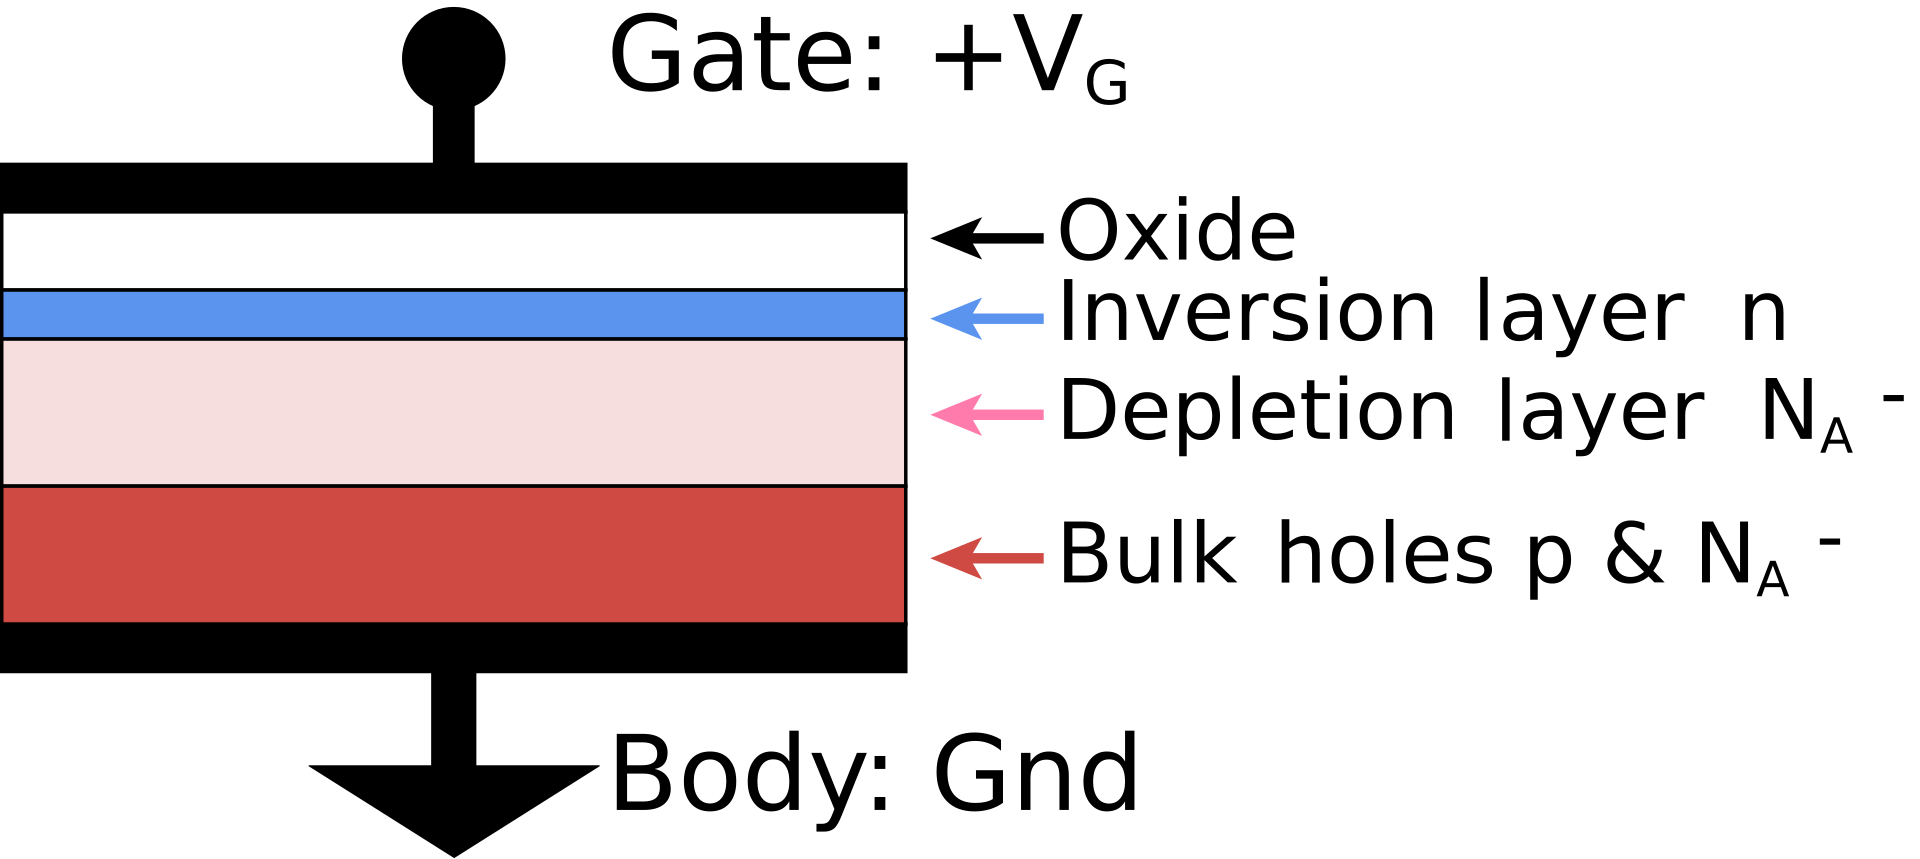
\includegraphics[width=0.5\textwidth]{MOS_Capacitor.png}
		\caption{A MOS capacitor (MOSCAP). Image by Brews ohare — Own work. Licensed under CC BY-SA 4.0, via Wikimedia Commons.
		}
		\label{fig:mosfet}
	\end{figure}
	When a voltage is applied to the gate, holes in the body, the p-type substrate, will be repelled, and minority electrons will be attracted, generating a depletion layer underneath the oxide layer. If the voltage is great enough, enough electrons will be attracted, and electrons become the majority carriers, forming an n-type region. We call this layer an \textbf{inversion layer}. The threshold voltage at which this happens is an important parameter. It is defined as that voltage, at which the density of the electrons in the inversion layer is the same as that of the density of holes in the p-type substrate. 
	
	If in addition, two so-called \textbf{terminals} are included on either side of the body, consisting of n-doped regions (opposite type compared to the body type), the source, and the drain, we call the structure a \textbf{MOSFET}. In the case of a p-type (n-type) body, and two n-type (p-type) terminals, we denote it an nMOSFET (pMOSFET)  or n-channel MOSFET. This makes up two pn-junctions. As voltage is applied to the gate and the inversion layer forms, a channel is formed that will allow current flow. The higher the voltage the greater the electron carrier density, and hence the greater the current flow between the two terminals. Transistors either amplify or switch electronic signals, and are essential building blocks in electronics. 
	
	\subsection{CCD charge generation during exposure of the camera}
	We are now ready to describe charge generation in the CCD pixel. Before exposure of the CCD, the MOSCAPs in the array are biased into the depletion region, thus having not formed the inversion layer at this point. The gate is then biased positively (in n-channel MOSCAPS) above the threshold for inversion, creating an n-channel below the gate, just as in the MOSFET structure. Holes are pushed far into the body substrate, and no mobile electrons remain; the CCD is in a non-equilibrium state called \textbf{deep depletion}. Now the chip is ready to detect photons, and formally the exposure begins. 
	
	As photons strike the depletion region, an electron-hole pair is formed and separated by the electric field. Charge is hence accumulated at the surface. This charge generation process can occur until a new thermal equilibrium is reached, a state which we call \textbf{full well}. The full well is a saturation effect, after which electrons may spill into neighboring pixels. The latter effect is called bleeding. This does not necessarily coincide with digital saturation, at which conversion of the signal from a current to a digital signal, in the analogue-to-digital converter, saturates due to lack of available bits. 
	
	Electron-hole pairs may also be created by thermal excitations anywhere in the array, generating noise referred to as dark current. This effect is linear with time and follows a Poisson distribution since they are rarely occurring stochastic incidents. Dark may be corrected for and is a crucial part of the characterization procedure.  
	
	\subsection{CCD charge transfer and image readout}
	After the phase of charge generation, usually called \textbf{exposure}, the accumulated charge must be read and interpreted as a digital signal in the computer. This digital signal should ultimately result in a value in each pixel. This is done by transferring the charge from the array, and sending the resulting electrical signal through an \textbf{analog-to-digital converter (ADC)} which will convert the analog signal of charges into a digitized signal that can be interpreted by a computer. This stage is called readout and happens on a line-by-line basis \footnote{Here a line denotes a row in the CCD MOSCAP array}. Rows are shifted down one at a time until they reach the \textbf{readout register} (the final row). Within each row, each pixel is read out sequentially.  
	
	Generally, during readout, the chip is exposed to light, and hence the shifting process should be very fast, to avoid smear in the image. This however poses another problem, as a faster readout process results in a higher noise level. This issue is solved in a \textbf{frame transfer CCD} by a shielded area of the chip, equal in size to the photosensitive area. The shielded area typically consists of a highly reflective material, such as aluminum. After exposure, the rows are rapidly shited into the shielded area, after which the necessary time to read out the measurements is available. In many cameras, this can also be achieved via a \textbf{mechanical shutter}. The camera used to develop the test procedure does not have a mechanical shutter, and we should hence characterize any potential time offset that may occur as a result of this.
	
	Now that a full description of CCD physics, and how a photosensitive detector works, has been presented, the basis of the testing procedure will be presented in the next section.
	
	\section{Characterization of CCDs}
	In order to determine if a CCD can meet the specified scientific goals of a mission, it must first be characterized. A characterization procedure is to be developed, and the result of that procedure applied to a detector, is to be compared to the scientific goals. The central characterization metrics of a CCD detector will be outlined in the following section. 
	
	\subsection{Gain}
	We shall begin by describing the most basic metric that related the digitized signal to the analog. The relationship between the number of electrons generated at the chip, and the actual pixel value in the image, is called \textbf{gain}\cite{handbookofccdastronomy}. This value is dependent on the software used to read out as well as the chip itself. As electrons are transferred out from the chip, they pass through an amplification stage, where a capacitor is charged. ´The voltage from this capacitor is passed through an \textbf{Analogue-to-digital converter (ADC)} which transforms the voltage signal into one that can be interpreted as a string of binary digits. This conversion is done by the software, and the resultant units are \textbf{Analogue-to-digital units (ADUs)}, which is ultimately the pixel value. At the ADC and software conversion levels we can scale the signal by an arbitrary factor, preserving the relative pixel values. This arbitrary scaling factor is exactly the gain. It can be expressed as
	\begin{equation}
		\text{gain} = \frac{\text{Number of electrons per pixel}}{\text{Number of counts per pixel}}
	\end{equation} 
	In each pixel bin on the chip, there is a maximum number of electrons that can be stored. This number is known as the \textbf{ful well capacity} of the chip. In addition, there is a maximum number that can be represented in the digitized signal, that depends on the number of available bits in the ADC. For a $16$bit ADC, this number is $\text{ADU}_{\text{max, 16 bit}} = 2^{16} = 65563$. It is hence natural to choose the gain factor, such that the full well capacity, corresponds to the maximum digital value that we can store. This is not necessarily the case as doing so can be difficult, as it relies on knowing this parameter to sufficient precision.
	
	\subsection{Dark frames}
	An intermediate definition is needed before we move on to the effects that require us to study the inherent behavior of the chip when not exposed to light, such as noise. A dark frame is an image acquired while the chip is not exposed to incoming photons. Such a frame may be used to study dark current and readout noise effects in a CCD detector and is also used to construct the master bias frame discussed below.
	
	\subsection{Bias}
	Readout noise in the chip follows a gaussian distribution (see section \ref{ron}) centered on zero. Hence there will be negative values in some of the pixels. To avoid negative counts in an image that consists entirely of noise, an offset voltage is applied to the CCD. This voltage offset level is called \textbf{bias}. 
	
	In general, bias is roughly constant across a chip, but it is common for the bias frame to show some level of structure in the chip. These structures can either be from the mechanical construction of the chip surface, from bad columns that may have a significantly higher offset than the rest of the chip, or resulting from the chip being made up of different sections that were constructed independently, and then later joined together. 
	
	Bad columns and sectors in the bias image are generally stable over a long time, and bias does not vary with time, and hence is independent of exposure time. 
	
	To study the bias level in the CCD, one may acquire an image with effectively zero exposure time\footnote{By effectively zero we mean, as short an exposure time, as is permitted by the camera at hand. Typically this value is in the range of about $0.001$s, which is also the case for the camera used to develop the testing procedure.}. In addition, this exposure should be a so-called \textbf{dark frame}. Such a frame is acquired in a dark setting such that no light reaches the chip during exposure or readout. Since the chip is initially discharged right before exposure, and then read out sequentially after the exposure has been completed, it is important to ensure that as few photons as possible reach the chip.
	
	This bias voltage must be characterized by acquiring dark frames. Such a bias voltage should be subtracted from other images when analyzing data, since it is an effect that is artificially introduced.
	
	\subsection{Noise}
	For a CCD there are three main types of important noise that must be characterize. These are \textbf{Readout noise (RON)}, \textbf{Photonic noise} and thermal noise also called \textbf{dark current}. These three kinds of noise will be discussed in turn below. 
	
	\subsubsection{Readout noise}\label{ron}
	Readout noise is the stochastic process associated with the amplification of the signal. It is introduced at the amplifier during the readout of the charge from the chip. It is usually quoted in terms of the number of an RMS number of electrons introduced per pixel upon readout \cite{handbookofccdastronomy}. Read noise cannot be eliminated, but it can be minimized. 
	
	There are two components to the phenomena. The first one is an introduction of uncertainty at the ADC level. The process of converting the analog signal to a digital one is not perfectly repeatable but is a distribution of possible answers centered on a mean value.
	The second component is extra electrons introduced by the electronics at work during readout. The width of the resultant additive distribution is interpreted as the readout noise, as a number of introduced electrons per pixel.
	The size and temperature of the amplifier contribute to this noise. Especially the temperature introduces as significant contribution due to thermal fluctuations. 
	
	Read-out noise follows a Gaussian distribution, and the width, that is the standard deviation of the distribution, is the read noise (in electrons) divided by the gain (in electrons per count). This can be seen by producing a histogram of the values in the master bias frame. It is seen that this distribution is gaussian with a mean value of the mean bias level offset, and a width corresponding to the readout noise. See figure \ref{fig:rongauss}. 
	
	\begin{figure}[h!]
		\centering
		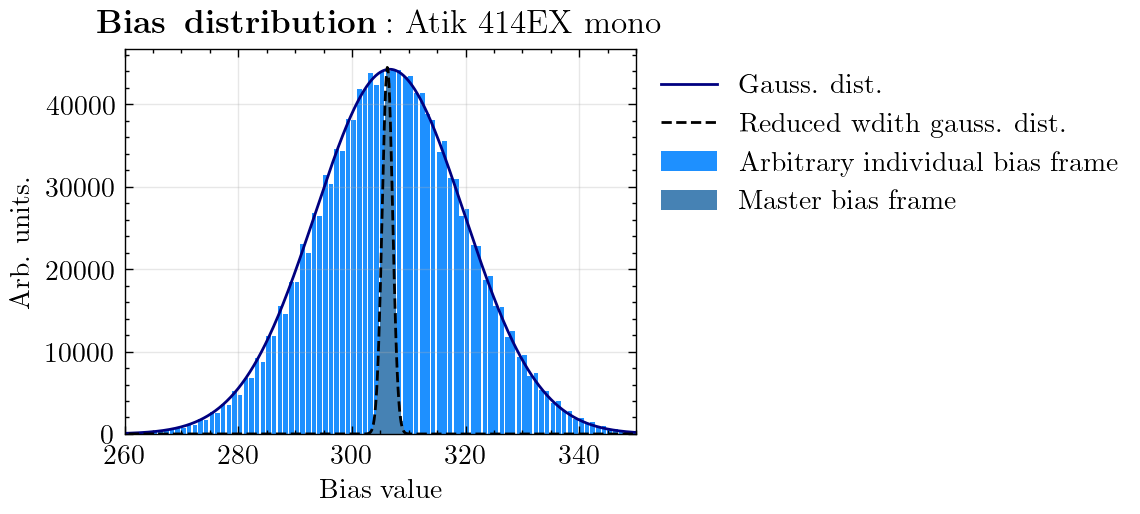
\includegraphics[width	=0.95\textwidth]{gauss_bias.png}
		\caption{}
		\label{fig:rongauss}
	\end{figure}
	
	Generally, a slower read-out speed will reduce the read-out noise \cite{handbookofccdastronomy}. This poses another complication, as a slower readout speed will introduce artifacts in the image, in the form of streaks, if the chip in question does not have a mechanical shutter.  
	
	\subsubsection{Photonic noise}
	Photon noise is the natural variation, or in other words statistical fluctuation, of the photonic flux detected by the CCD. Photons detected follow a poisson distribution, since each photon is a discrete quanta, and the probability of the detection of the photon is independent of the other photons detected. A poisson distribution tends to that of normal distribution for large numbers, and hence the photon noise depends on the number of photons detected. We may hence reduce this photonic noise by observing bright objects that emit many photons, or by using longer exposure times.
	
	\subsubsection{Thermal noise and Dark current}
	Thermal noise, also called \textbf{dark current} is the resulting current in the chip, due to the thermal motion of the electrons in the solid-state material. This effect can be studied using the so-called \textbf{dark-frames} described above, in which the chip is not exposed to incoming photons, and hence no photo-electrons should be produced (in the ideal case of a perfectly dark room). The dark current depends linearly on time and is usually given as electrons per second. We thus obtain the following relation for the dark current in the chip
	
	\begin{equation}\label{darkcurrenteq}
		\text{dark current} = \frac{\text{ADU} * \text{gain}}{\text{exposure time}},
	\end{equation}
	
	where the ADU value refers to the mean ADU / pixel in a dark frame. Gain is the detector gain described above. Thermal noise contaminates astronomical images making them hard to analyze and interpret scientifically, and should be eliminated. Fortunately, since dark current results from the thermal motion of electrons in the chip, it is strongly temperature-dependent and can be practically eliminated by cooling the chip. A well-designed testing procedure should characterize the dark current levels as a function of temperature. Readout noise levels are usually significantly greater than dark current levels, so dark frames must be taken at long exposure times, to yield an appreciably large dark current effect that can be practically isolated from that of the readout noise. This can also be achieved by averaging over a large number of dark frames, to average out readout noise. It should also be noted that a master bias frame should be subtracted from the dark fame to isolate dark current levels. 
	
	A master dark current frame can be constructed by averaging over many dark frames at a given exposure, subtracting the master bias frame, and then computing the dark current in each pixel according to equation \ref{darkcurrenteq}. Such a frame can be seen in \ref{fig:masterdarkcurrent}.
	\begin{figure}[h!]
		\centering
		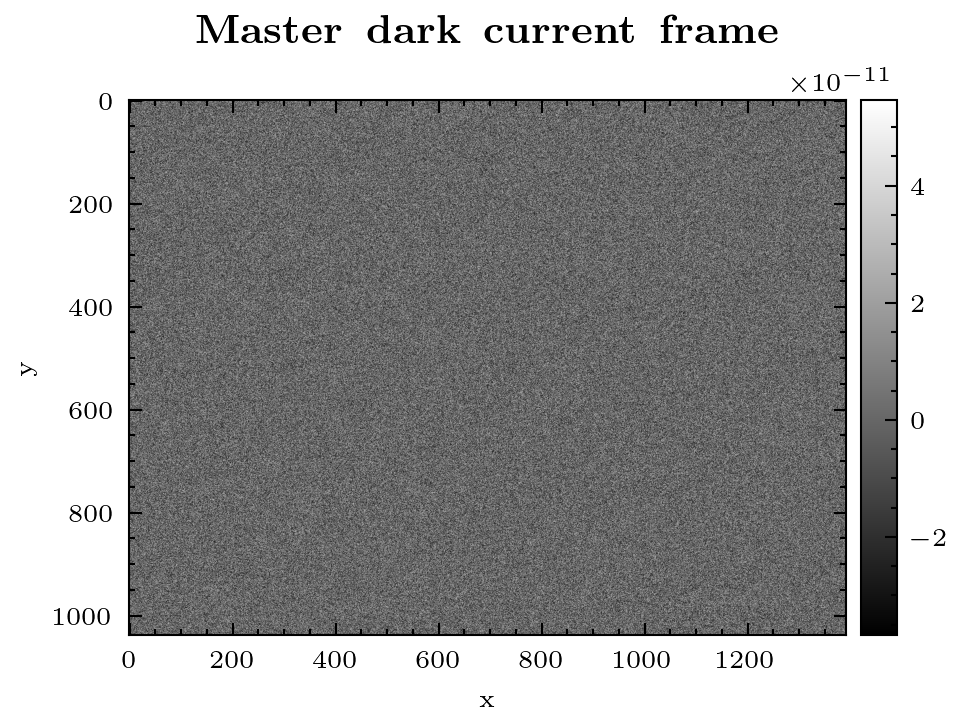
\includegraphics[width	=0.95\textwidth]{master_dark.png}
		\caption{A master dark current frame constructed by averaging over many dark frames at a given exposure, subtracting the master bias frame, and then computing the dark current in each pixel according to equation \ref{darkcurrenteq}.}
		\label{fig:masterdarkcurrent}
	\end{figure}
	
	\subsection{Flat fielding}\label{sec:flat}
	A CCD may not have a perfectly flat response to incoming light. By an ideal flat CCD detector, we mean a detector that uniformly detects photons with the same efficiency and sensitivity across the entire photo-active region of the chip. This ideal situation is seldom realized in practice due to faults in the chip or various manufacturing processes. Some CCDs may be constructed by joining several photo-sensitive pieces of silicon or may be constructed by grinding off layers of a block of silicon to achieve a thin detector. This grinding process may leave circular or straight lines through the chip that can be either more or less sensitive to light. There may also be specks of dust or fingerprints on the camera window causing blocking of light and diffraction patterns in the image.
	
	In order to overcome this difficulty and to reconstruct the desired image from detector data in a non-flat CCD (which is usually the case at hand), we can utilize flat-field frames. Such frames are acquired by imaging a flat field, such as a white flat screen. Any non-uniformities in the resulting image, should, in the ideal experimental design, be due to the non-flatness of the chip, or obstructing objects on the camera window. This flat field frame then represents the relative light sensitivity between pixels in the chip. Construction of a master flat-field frame, by averaging over many such flat exposures, can then be used as a correction frame after normalizing it to unity. This is done by finding the greatest pixel ADU-value in the array and dividing the rest of the pixels in the frame by this value. This should be done after a hot pixel correction that will be described below. Now the master flat contains values in the interval (0, 1], the right end of the interval representing pixels that receive the most light. This frame can now be used for flat field corrections. This is done by dividing an image in question with the master flat on a pixel-by-pixel basis \footnote{Division by zero will not be a problem in practice, since generally there will always be a non-zero value in each pixel, for an arbitrary exposure time greater than bias, even after bias correction.}. An example of such a master flat frame can be seen in figure \ref{fig:masterflat}.
	
		\begin{figure}[h!]
		\centering
		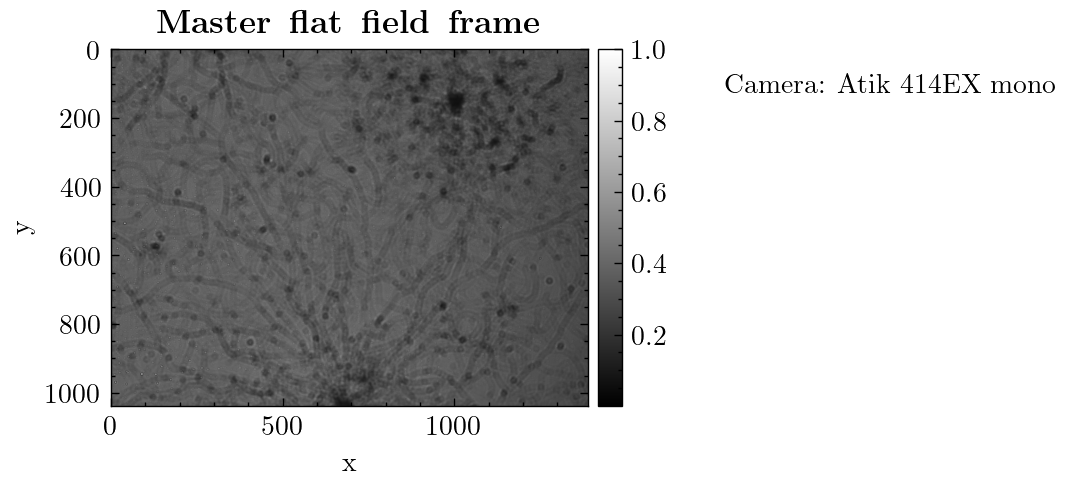
\includegraphics[width	=0.95\textwidth]{master_flat.png}
		\caption{A master flat frame constructed by averaging over a given number of light exposures of a flat field, with $10s$ exposure times, subtrcting the bias and dark current master frames, and then normalizing to unity as described in section \ref{sec:flat}. }
		\label{fig:masterflat}
	\end{figure}
	
	\subsection{Hot pixels}
	A hot pixel is one which after an arbitrary exposure time, has an ADU value that is significantly greater than the mean value in the image. Such an effect can occur either because that pixel has a higher sensitivity to incoming photons due to the detector being struck by cosmic rays, or because the dark current in that pixel is higher and/or not proportional to time in a linear way. Dealing with cosmic rays is of particular importance for cameras in space since the rate of incidence is much higher than at the surface of the earth.
	
	\subsection{Linearity}
	Linearity is the response between measured ADUs and exposure time. In other words, if one doubles the exposure time, we expect to double the number of measured ADUs. We may study this effect by acquiring frames at different exposure times and comparing the mean ADU/pixel across exposure times. A detector is seldom perfectly linear, and the non-linearity must therefore be characterized. This is crucial for astronomical purposes since many observational metrics depend on the flux. In observing a star, using the passage method to detect exo-planets, the size of a planet can be estimated from the periodical dip in flux. If the detector, for a given exposure time (or equivalently ADU-range) is non-linear, the dip in flux will be affected, and the size of the planet may be larger or smaller. 
	
	The non-linearity of the detector may be defined as the deviation of a given measurement from the perfect linear behavior.
	
	\subsection{Charge diffusion and charge transfer efficiency}
	
	
\end{document}